% Transition diagrams of the four channels of notebook 50, Section 5.1: noiseless, binary symmetric (flip q),
% binary erasure (erasure e, output '?'), Z-channel (input 1 becomes 0 with probability s). Arrows carry P(y|x);
% below each diagram, the stochastic matrix W with rows x and columns y (rows sum to one).
\documentclass[tikz,border=6pt]{standalone}
\usepackage{amsmath,amssymb}
\usetikzlibrary{arrows.meta,positioning,calc}
\begin{document}
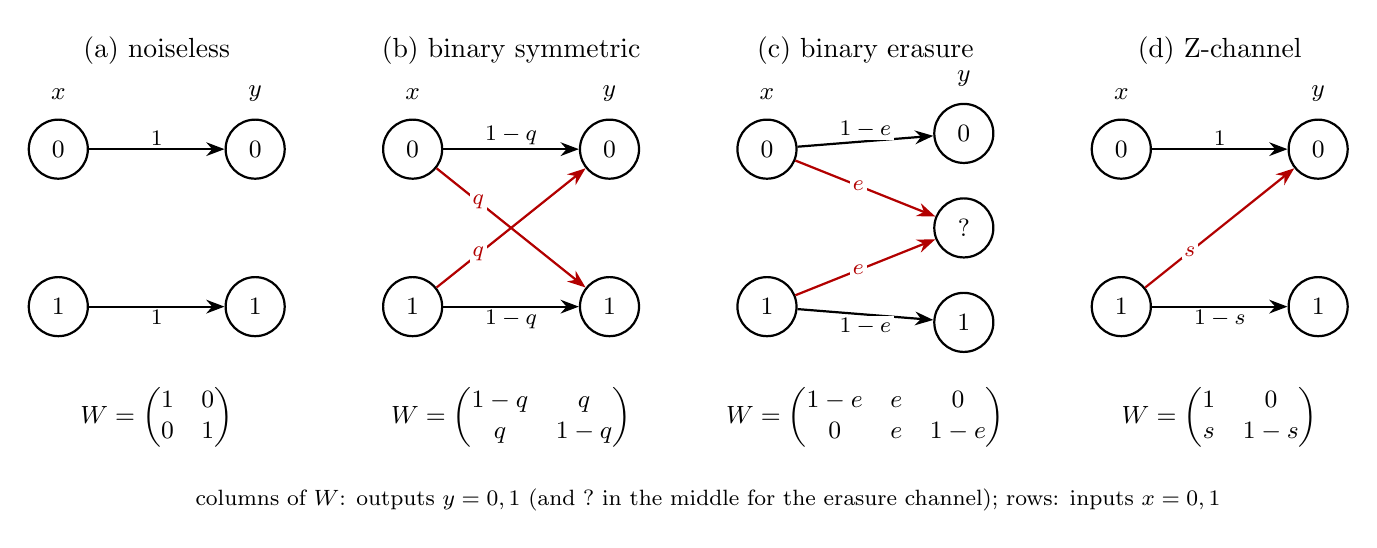
\begin{tikzpicture}[thick, >=Stealth, font=\small,
    sym/.style={circle, draw, fill=white, minimum size=0.75cm, inner sep=0pt},
    lab/.style={font=\footnotesize, fill=white, inner sep=1pt}]
  % ---- (a) noiseless
  \begin{scope}[shift={(0,0)}]
    \node[font=\normalsize] at (1.25,1.25) {(a) noiseless};
    \node[sym] (x0) at (0,0) {$0$}; \node[sym] (x1) at (0,-2) {$1$};
    \node[sym] (y0) at (2.5,0) {$0$}; \node[sym] (y1) at (2.5,-2) {$1$};
    \draw[->] (x0) -- node[lab, above] {$1$} (y0);
    \draw[->] (x1) -- node[lab, below] {$1$} (y1);
    \node at (0,0.7) {$x$}; \node at (2.5,0.7) {$y$};
    \node at (1.25,-3.4) {$W=\begin{pmatrix}1&0\\0&1\end{pmatrix}$};
  \end{scope}
  % ---- (b) BSC
  \begin{scope}[shift={(4.5,0)}]
    \node[font=\normalsize] at (1.25,1.25) {(b) binary symmetric};
    \node[sym] (x0) at (0,0) {$0$}; \node[sym] (x1) at (0,-2) {$1$};
    \node[sym] (y0) at (2.5,0) {$0$}; \node[sym] (y1) at (2.5,-2) {$1$};
    \draw[->] (x0) -- node[lab, above] {$1-q$} (y0);
    \draw[->] (x1) -- node[lab, below] {$1-q$} (y1);
    \draw[->, red!70!black] (x0) -- node[lab, pos=0.28] {$q$} (y1);
    \draw[->, red!70!black] (x1) -- node[lab, pos=0.28] {$q$} (y0);
    \node at (0,0.7) {$x$}; \node at (2.5,0.7) {$y$};
    \node at (1.25,-3.4) {$W=\begin{pmatrix}1-q&q\\q&1-q\end{pmatrix}$};
  \end{scope}
  % ---- (c) BEC
  \begin{scope}[shift={(9.0,0)}]
    \node[font=\normalsize] at (1.25,1.25) {(c) binary erasure};
    \node[sym] (x0) at (0,0) {$0$}; \node[sym] (x1) at (0,-2) {$1$};
    \node[sym] (y0) at (2.5,0.2) {$0$}; \node[sym] (ye) at (2.5,-1) {$?$}; \node[sym] (y1) at (2.5,-2.2) {$1$};
    \draw[->] (x0) -- node[lab, above] {$1-e$} (y0);
    \draw[->] (x1) -- node[lab, below] {$1-e$} (y1);
    \draw[->, red!70!black] (x0) -- node[lab, pos=0.45] {$e$} (ye);
    \draw[->, red!70!black] (x1) -- node[lab, pos=0.45] {$e$} (ye);
    \node at (0,0.7) {$x$}; \node at (2.5,0.9) {$y$};
    \node at (1.25,-3.4) {$W=\begin{pmatrix}1-e&e&0\\0&e&1-e\end{pmatrix}$};
  \end{scope}
  % ---- (d) Z-channel
  \begin{scope}[shift={(13.5,0)}]
    \node[font=\normalsize] at (1.25,1.25) {(d) Z-channel};
    \node[sym] (x0) at (0,0) {$0$}; \node[sym] (x1) at (0,-2) {$1$};
    \node[sym] (y0) at (2.5,0) {$0$}; \node[sym] (y1) at (2.5,-2) {$1$};
    \draw[->] (x0) -- node[lab, above] {$1$} (y0);
    \draw[->] (x1) -- node[lab, below] {$1-s$} (y1);
    \draw[->, red!70!black] (x1) -- node[lab, pos=0.3] {$s$} (y0);
    \node at (0,0.7) {$x$}; \node at (2.5,0.7) {$y$};
    \node at (1.25,-3.4) {$W=\begin{pmatrix}1&0\\s&1-s\end{pmatrix}$};
  \end{scope}
  \node[font=\footnotesize] at (8.25,-4.45) {columns of $W$: outputs $y=0,1$ (and $?$ in the middle for the erasure channel); rows: inputs $x=0,1$};
\end{tikzpicture}
\end{document}
